\section{Architectures de cartes auto-organisatrices}

Ainsi, cette thèse se place dans une démarche de construire un modèle d'architecture permettant un calcul émergent, à partir de cartes auto-organisatrices.

Les cartes auto-organisatrices ont été largement étudiées depuis leur introduction en 1984. On dénombre de milliers de papiers en traitant, rien que sur la période 1984 - 2003 pour laquelle une bibliographie exhaustive par mot clés a été menée par Lampinen et Oja (ref). De nombreux papiers ont été publiés depuis, 10000 selon une recherche par mot clés sur google scholar. 

La question d'architecture de cartes de Kohonen a été explorée. Associer les cartes en modèle hiérarchique faisait même partie des premiers travaux publiés autour des cartes de Kohonen.
L'association de quelques cartes de Kohonen dans des applications spécifiques est également assez répandue:
(citer association de cartes pour détection d'erreur, autres applis ?). Tous ces modèles sont des constructions adaptées pour résoudre un problème de machine learning spécifique.

Mais étonnament peu de travaux, par rapport à la littérature sur le sujet, se sont intéressés à l'association de cartes en tant que nouveau modèle à part entière.

Dans cette section, nous passons en revues les modèles existantes permettant, d'une façon ou d'une autre, de connecter des cartes entre elle. Nous étudierons d'un coté les modèles d'architectures de plusieurs cartes communiquant via des interfaces; nous étudierons également les modèles de cartes récurrentes. Les cartes récurrentes sont appliquées à des motifs temporels et ont la caractéristique d'utiliser des éléments de leur état passé pour calculer leur état à un instant donné. La notion de communication est ici encore présente et peut nous servir d'inspiration pour développer une architecture de cartes. Par ailleurs, nous avons mentionné que le traitement de données temporel doit pouvoir être intégrée dans une architecture de carte visant à être autonome. Il s'agit ici de trouver une méthode d'interface entre carte qui puisse à la fois connecter des cartes auto-organisatrices et introduire des connections récurrentes dans le temps. 

\subsection{Modèles de SOM impulsionnelles}

De nombreux travaux de biologie observent des co-activations entre les zones du cerveaux. Le cortex cérébral est ainsi être considéré comme un reseaux de neurone modulaires, avec des régions s'activant entre elles. \cite{primate_cortex_91,mountcastle_columnar_1997,Harriger2012RichCO}

Ces coactivations aient été observées expérimentalement. Plusieurs modèles en neurosciences computationnelles ont été proposés pour expliquer ce phénomènes. Les modèles les plus communs sont la zone de convergence-divergence de Damasio (CDZ) \cite{damasio_time-locked_1989}, et le modèle de boucles de réentrées de Edelmann \cite{Edelman1982GroupSA}.

La zone de convergence divergence propose que certains réseaux de neurones dans le cerveau servent de connexions pour associer d'autres zones corticales. Lorsque cette zone est excitée par des signaux en provenance d'une zone corticale, elle propage cette excitation vers les autres zones.
La théorie de la ré-entrée postule quant à elle des connexions directes et réciproques entre  les neurones de différentes cartes cérébrales. Ces connexions permettent la coactivation de neurones dans différentes cartes. 

Par leur proximité avec la biologie, les travaux sur les réseaux de neurones impulsionnels ont été plus encleins à développer des modèles de cartes connectées, s'inspirant notamment des deux théories de convergence-divergence et de réentrée. Le fait que ces réseaux reposent déjà sur des calculs locaux les rendent de bons candidats pour créer des réseaux modulaires. En \cite{electronics9101605}, les auteurs passent en revue différents modèles implémentant de telles architectures au vu de leur plausibilité biologique, et proposent également une architecture de deux cartes auto-organisatrices impulsionnelles pour faire de la fusion de données.

\subsection{The hierarchical self organizing map}

Contrairement aux réseaux impulsionnels qui utilisent des règles d'activation à l'échelle d'un neurone, les cartes auto-organisatrices (SOM) et de ses variantes (GSOM, Tree SOM) définissent des règles de calcul à l'échelle de la carte.
 Ces calculent s'appuient sur sur des distances et un principe de voisinage, imitant finalement des règles locales; on parle ainsi de processus d'auto-organisation. Les motifs d'activation qu'ils développent sont similaires à ceux que l'on retrouve dans des zones cérébrales telles que le cortex visuel.

Il est donc pertinent d'étudier comment plusieurs cartes auto-organisatrices peuvent être connectées pour réaliser un calcul décentralisé.
De nombreux travaux utilisent des modèles incluant plusieurs cartes auto-organisatrices; mais la plupart de ces architectures sont conçues pour une application spécifique.
On ne peut donc pas parler de modèles modulaires. Certains travaux ont cependant développé des modèles modulaires conçus en combinant les cartes comme un nouveau modèle générique et exploiter les communications.

Dès que les SOMs ont été introduites, des version hiérarchique a été proposée, HSOM : \cite{lampinen_clustering_1992,koikkalainen_self-organizing_1990} . Dans HSOM, une carte apprend des données comme une première couche et transmet l'index de son BMU comme entrée à une deuxième carte. Les auteurs ont observé que la deuxième carte a une capacité de regroupement plus précise qu'une seule carte. Certaines variantes de HSOM ont été proposées par la suite, comme l'arbre d'architecture croissante soms [ref], où l'architecture hiérarchique est de plus en plus conçue pour s'adapter à l'ensemble des données. Dans ce cas, l'activité entière d'une carte est transmise en entrée aux couches supérieures. (Citons également [baruque])
Ces architectures hiérarchiques ont principalement pour but d'amélorier les capacités d'organisation des cartes.

% \subsection{Modèles de cartes, mémoire associative}


% D'autre part, certains travaux visent à connecter les cartes entre elles de manière directe, en se rapprochant de la théorie de la rentrée d'Edelman. C'est le cas de A-SOM : combiner des cartes. \cite{johnsson_associative_2009}.

% Certains travaux développent des cartes modulaires où les connexions entre cartes sont créées neuronalement. C'est le cas de l'algorithme SOIMA \cite{SOIMA}, où les connexions entre neurones sont apprise avce une regle hebbienne alors que l'apprentissage se fait dans chaque carte : les neurones qui s'activent ensemble voient leur poids de connexion renforcé.

\subsection{Modèle CDZ de Dominey}

Dans \cite{dominey13}, les auteurs construisent des architectures hiérarchiques en transmettant les positions des BMU entre les cartes multimodales. L'inspiration est tirée du cadre CDZ.
Chacune des cartes possède plusieurs couches, chacune prenant une modalité en entrée. Une activité est calculée sur ces modalités en une activité commune. La position du BMU, en l'occurence un vecteur 3D, sera utilisée comme modalité hiérachique pour connecter des cartes entre elle. Dans ces travaux, les auteurs présentent une architecture hiérarchique, en s'appuyant sur le modèle CDZ. Une carte amodale sert alors à connecter des cartes modales.
Dans le cas d'une hiérarchie de cartes, les auteurs entrainent les couches de l'architecture séparément: les cartes modales du premier niveau sont apprises, puis la carte amodale les connectant est apprise dans un second temps. 
Une fois toute les cartes apprises, la structure est utilisée pour activer une ou des modalités en activant la carte amodale. Cette carte représente la zone de convergence divergence des modèles cérébraux. 

Ce modèle se rapproche fortement du modèle HSOM de 1992; la différence réside dans le fait de réaliser des cartes à plusieurs modalités, et 'd'utiliser la hiéarchie pour associer des cartes de modalités. 
L'utilisation de la position du BMU en tant que vecteur transmis entre carte est une bonne compression de l'information d'une modalité.

\begin{figure}
    \centering
    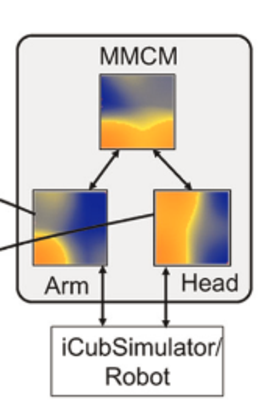
\includegraphics[width=0.3\textwidth]{MMCM_schema.pdf}
    \caption{Architecture MMCM. Les cartes du premier niveau recoivent l'une les mouvements de tête d'un robot, l'autre les mouvements de main. Les cartes convergent en une carte amodale (MMCM). L'activation de cette carte produit des mouvements coordonées tête/mains~\cite{dominey13}\label{fig:mmcm}}
\end{figure}

\subsection{A-SOM}





\section{Cartes auto-organisatrices récurrentes}

On appelle réseaux récurrents des réseaux de neurones qui prennent en compte leur état précédent pour calculer leur état actuel. Ces réseaux sont utilisés pour le traitement et l'apprentissage de signaux temporels. Citons par exemple, en deep learning, les RNN (recurrent neural networks), dont les neurones recoivent leur état précédent en entrée. Les réseaux récurrents les plus utilisés actuellement sont les LSTM, dans lesquel un système de portes perment d'activer ou non des neurones en fonction des états précédents du réseau. Les cartes de Kohonen ont elles aussi des version récurrentes que nous allons présenter dans cette partie.

Nous nous intéressons aux architectures multi-cartes, mais les cartes récurrentes répondent à des problèmes très similaire à ceux rencontrés dans la conception d'architectures de cartes pour faire de la mémoire associative. Dans une carte récurrente, le problème principal est de trouver comment communiquer à la carte de l'information sur son état précédent et comment utiliser cette information dans l'apprentissage de l'état courant. Cela rejoint la problématique posée dans les architectures de cartes de Kohonen, qui est de comment communiquer à une autre carte son état, afin de l'utiliser dans l'apprentissage de l'état courant. Nous avons vu précedemment qu'il existe assez peu de modèles d'architectures de cartes. Il existe plusieurs modèles de carte récurrentes qui nous permettrons de compléter cette étude. 

Notre volonté de créer un modèle général d'architecture de cartes auto-organisatrice motive également le fait de s'intéresser aux cartes récurrentes. On souhaite en effet créer un modèle qui puisse unir cartes récurrentes et cartes normales au sein d'une même architecture. L'aspect bio-inspiré du modèle et son aspect multimodal ciblent plutot des applications d'un tel réseau en robotique. Or, la plupart des données traitées par des réseaux de neurones, en particulier dans les applications robotiques, sont temporelles : vidéos, signaux sonores, capteurs de position. Il est donc important de s'appuyer autant sur les modèles de cartes récurrentes existantes que sur les architectures afin de créer un modèle général. 

%Enfin, les cartes de Kohonen ne se prêtent pas à un apprentissage en ligne de données en temps réel. En effet, il est nécessaires que les données d'entrées soient tirées aléatoirement dans l'espace à apprendre et ne suivent pas une trajectoire. Par exemple, si on veut apprendre des images, mais que les entrées sont données à la carte sous la forme d'une vidéo, les frames de la vidéo sont proches les unes des autres et forment donc une continuité dans l'espace d'entrée des images à apprendre. La carte va alors apprendre le sous ensemble de l'espace sur lequel se trouvent les premières frames, puis les oublier au fur et à mesure de l'apprentissage et les remplacer par les images qui suivent. Avec une architecture multi cartes qui prendrait en compte un aspect temporel, on pourrait imaginer la construction d'une architecture plus robuste.

Nous avons classé les modèles de cartes récurrentes existants en différentes catégories. D'une part, certains modèles de cartes utilisent l'état précédent de la carte lors du calcul de l'activité de l'état courant. De l'autre, des modèles réutilisent plutot des élement de la carte précedente en tant qu'entrée de l'état courant.


\subsection{Cartes récurrentes }

\draft{TKM, RSOM, utilisation seulement de la zone autour du BMU}


\subsection{The Hypermap architecture, TKM, RSOM}
Parmi les premiers travaux autour des cartes auto-organisatrices, Kohonen propose l'"Hypermap". L'idée de cette méthode est, pour une carte apprenant sur une séquence d'entrée, de présenter la carte une entrée et un contexte dépendant de l'état précédent. Ce contexte défnit une zone de la carte dans laquelle faire le matching.

\subsection{MSOM}
